%
% pef.tex (LateX)
% 
% Objetivo: Capítulo sobre o método de interpolação com filtros adaptativos de predição de erro
% (PEF, do inglês) do relatório de qualificação de doutorado.
% 
% Versão 1.0
% 
% Site: http://www.dirackslounge.online
% 
% Programador: Rodolfo A. C. Neves (Dirack) 17/10/2019
% 
% Email: rodolfo_profissional@hotmail.com
% 
% Licença: GPL-3.0 <https://www.gnu.org/licenses/gpl-3.0.txt>.

\chapter{FILTROS ADAPTATIVOS DE PREDIÇÃO DE ERRO (FPE)}
\label{cap4}

Uma restrição comumente utilizada na interpolação de traços sísmicos
é assegurar que os dados interpolados, depois da filtragem,
tenham mínima energia. Isto significa a escolha de valores
nos limites do filtro de modo a minimizar o transiente. Neste ponto os mínimos
quadrados levam grande vantagem, pois tendem a absorver grandes valores e a distribuir
uniformemente os resíduos em tempo e frequência na extensão permitida \cite{claerbout92}.

A filtragem é equivalente a multiplicação espectral. Assim, especificar a filtragem
é o equivalente a preescrever o espectro dos dados interpolados. Uma escolha sensível
é o espectro do dado registrado, que pode ser capturado através dos coeficientes dos
filtros adaptativos de predição de erro (FPE) do dado \cite{spitz}. 

Os FPE, também conhecidos como filtros de autoregressão, desenpenham o
papel da ``matriz inversa de covariância'' da teoria das estimativas na estatística.
O sinal é regredido sobre si mesmo na estimativa dos coeficientes do filtro. O FPE
pode ser implementado no domínio tempo-espaço ou frequência-espaço. Os FPE no tempo-espaço
são menos propensos a criar eventos espúrios na presença de ruído do que os filtros
frequência-espaço \cite{abma}. 

A utilização dos FPE na interpolação ocorre em dois passos:
Primeiro, o FPE é estimado através da minimização da saída da convolução
dos dados conhecidos com o FPE desconhecido. Segundo, os dados interpolados
são estabelecidos a partir da minimização da convolução do FPE anteriormente 
calculado com o modelo conhecido, restringido pelos dados conhecidos \cite{curry}.

Contudo, a busca dos coeficientes do FPE necessita evitar equações regressivas que 
envolvam as fronteiras ou dados ausentes. Isto pode ser feito
criando uma máscara de seleção $K(t,x)$, uma matriz 
diagonal de uns nos traços originais e zeros nos traços a serem interpolados, 
para translações causais e entradas de dados \cite{claerbout10}

Os coeficientes $B_n(t,x)$ do filtro são obtidos
solucionando o problema de mínimos quadrados \cite{liu11}:

\begin{equation}
\label{eq:4.1}
\hat{B_n}(t,x) = \arg \min_{B_n} \left \rVert K(t,x) \left [ S(t,x) - \sum^N_{n=1}B_n(t,x)S_n(t,x) \right ] \right \Arrowvert^2_2 
+ \epsilon^2 \sum^N_{n=1} \left \rVert D [ B_n(t,x) ] \right \Arrowvert^2_2
\end{equation}

Onde $S_n(t,x) = S(t-i,x-j)$, representa a tranlação causal de $S(t,x)$. 
$D$ é um operador de regularização e $\epsilon$ é um parâmetro de regularização escalar.

Se $D$ for definido como um operador linear, a estimativa através dos mínimos quadrados se reduz a uma
inversão linear \cite{liu11, fomel2009}.

\begin{equation}
\label{eq:4.2}
b = A^{-1} d
\end{equation}

Onde:

\begin{equation}
\label{eq:4.3}
 b = \left[ B_1(t,x)\:\: B_2(t,x)\:\: ...\:\: B(t,x) \right]^T
\end{equation}

\begin{equation}
\label{eq:4.4}
 d = \left[ S_1(t,x)S(t,x)\:\: S_2(t,x)S(t,x)\:\: ... \:\: S_N(t,x)S(t,x) \right]^T
\end{equation}

E os elementos da matriz $A$ são:

\begin{equation}
\label{eq:4.5}
 A_{nk}(t,x) = S_n(t,x)S_k(t,x) + \epsilon^2 \delta_{nk}D^TD
\end{equation}

Ao incorporar um operador de suavização $G$ ao invés de $D$ estabelecemos uma janela de suavização
dado o tamanho e a forma do filtro $B_n(t,x)$ e o raio da janela de suavização no espaço e no tempo em $G$ \cite{fomel2007}.
Os coeficientes do filtro nos traços zerados intercalados aos traços originais estão assim restringidos pelos limites
da janela de suavização, dando maior peso aos traços mais próximos.

Isto é feito definindo $G$ como um operador de suavização gaussiano com raio ajustável, obrido através da
aplicação repetida de um filtro triangular e da escolha do parâmetro $\lambda$ como o valor médio de $S_n(t,x)$.
Com estas considerações a inversão toma a forma \cite{liu11, fomel2007}:

\begin{equation}
\label{eq:4.6}
 b = \hat{A}^{-1}\hat{d}
\end{equation}

Onde:

\begin{equation}
\label{eq:4.7}
 \hat{d} = [ G[S_1(t,x)S(t,x)]\:\: G[S_2(t,x)S(t,x)]\:\: ...\:\: G[S_N(t,x)S(t,x)] ]^T
\end{equation}

Os elemetos da matriz $\hat{A}$ são:

\begin{equation}
\label{eq:4.8}
 \hat{A}_{nk}(t,x) = \lambda^2 \delta_{nk} + G[S_n(t,x)S_k(t,x) - \lambda^2 \delta_{nk}]
\end{equation}

A segunda etapa também é resolvida a partir dos mínimos quadrados. Porém,
o filtro já é conhecido e o objetivo agora é estimar os traços desconhecidos.
A partir da seguinte formulação de um novo problema de mínimos quadrados \cite{liu11}:

\begin{equation}
\label{eq:4.9}
 \hat{S}(t,x) = \arg \min_S \left \rVert S(t,x) - \sum^N_{n=1}\hat{B}_n(t,x) S_n(t,x) \right \Arrowvert^2_2
\end{equation}

Sujeito a seguinte restrição dos traços conhecidos:

\begin{equation}
\label{eq:4.10}
 \hat{S}(t,x) = S_{known}(t,x_k)
\end{equation}

Onde $\hat{S}(t,x)$ representa a saída da interpolação.
A minimização é feita a partir do método dos gradientes-conjugados \cite{hestenes}. 
A restrição a partir da Equação \ref{eq:4.3} é utilizada como modelo inicial e restringe
a saída utilizando os traços conhecidos em cada iteração no esquema dos gradientes-conjugados.
O custo computacional é proporcional ao número de iterações multiplicado
pelo tamanho do filtro, o número de amostras no tempo e no espaço $N_i \times N_f \times N_t \times N_x$. 
Crescendo o raio de suavização na regularização decresce o número de iterações no passo da
estimativa do filtro \cite{liu11}.

Os filtros adaptativos de predição de errro (FPE) podem ser utilizados para regularizar os dados sísmicos,
de modo a produzir uma amostragem suficiente para o estabelecimento das seções ERC.
Como representado na Figuras \ref{fig:4.1}, a trajetória ERC calculada para cada $m_0$ não
necessariamente intersecta as seções de afastamento constante nas coordenadas $m_i$, $h_i$ dos traços sísmicos. 
A trajetória ERC calculada passa entre os traços identificados pelas coordenadas $m1,h2$ e $m3, h2$ na Figura \ref{fig:4.1},
sendo necessário aumentar a discretização em $m$ da seção $h2$ para poder amostrar corretamente a trajetória ERC.

Ao intercalar os traços originais com novos traços zerados $m'_i$, e utilizar os filtros adaptativos de predição
de erro para interpolar os valores das amostras em cada traço $m'_i$, dobramos 
a discretização das seções de afastamento constante.
Este processo pode ser repetido até que a discretização seja suficiente para amostrar a curva ERC em cada seção de afastamento
constante (na Figura \ref{fig:4.2}, $m'_2$ está mais próximo da trajetória 
ERC do que $m_3$ e $m_2$ já que a distância 
entre os traços da seção $\Delta m$ é menor).

\begin{figure}
\caption{Representação esquemáticas de uma trajetória ERC para um $m_0$ arbitrário. A trajetória intersecta a seção de
afastamento constante entre dois traços sísmicos identificados pelas coordenadas $m2, h2$ e $m3, h2$, sendo necessário
aumentar a discretização para amostrar corretamente a trajetória. $\Delta m$ é a distância entre os traços da seção.}
\begin{center}
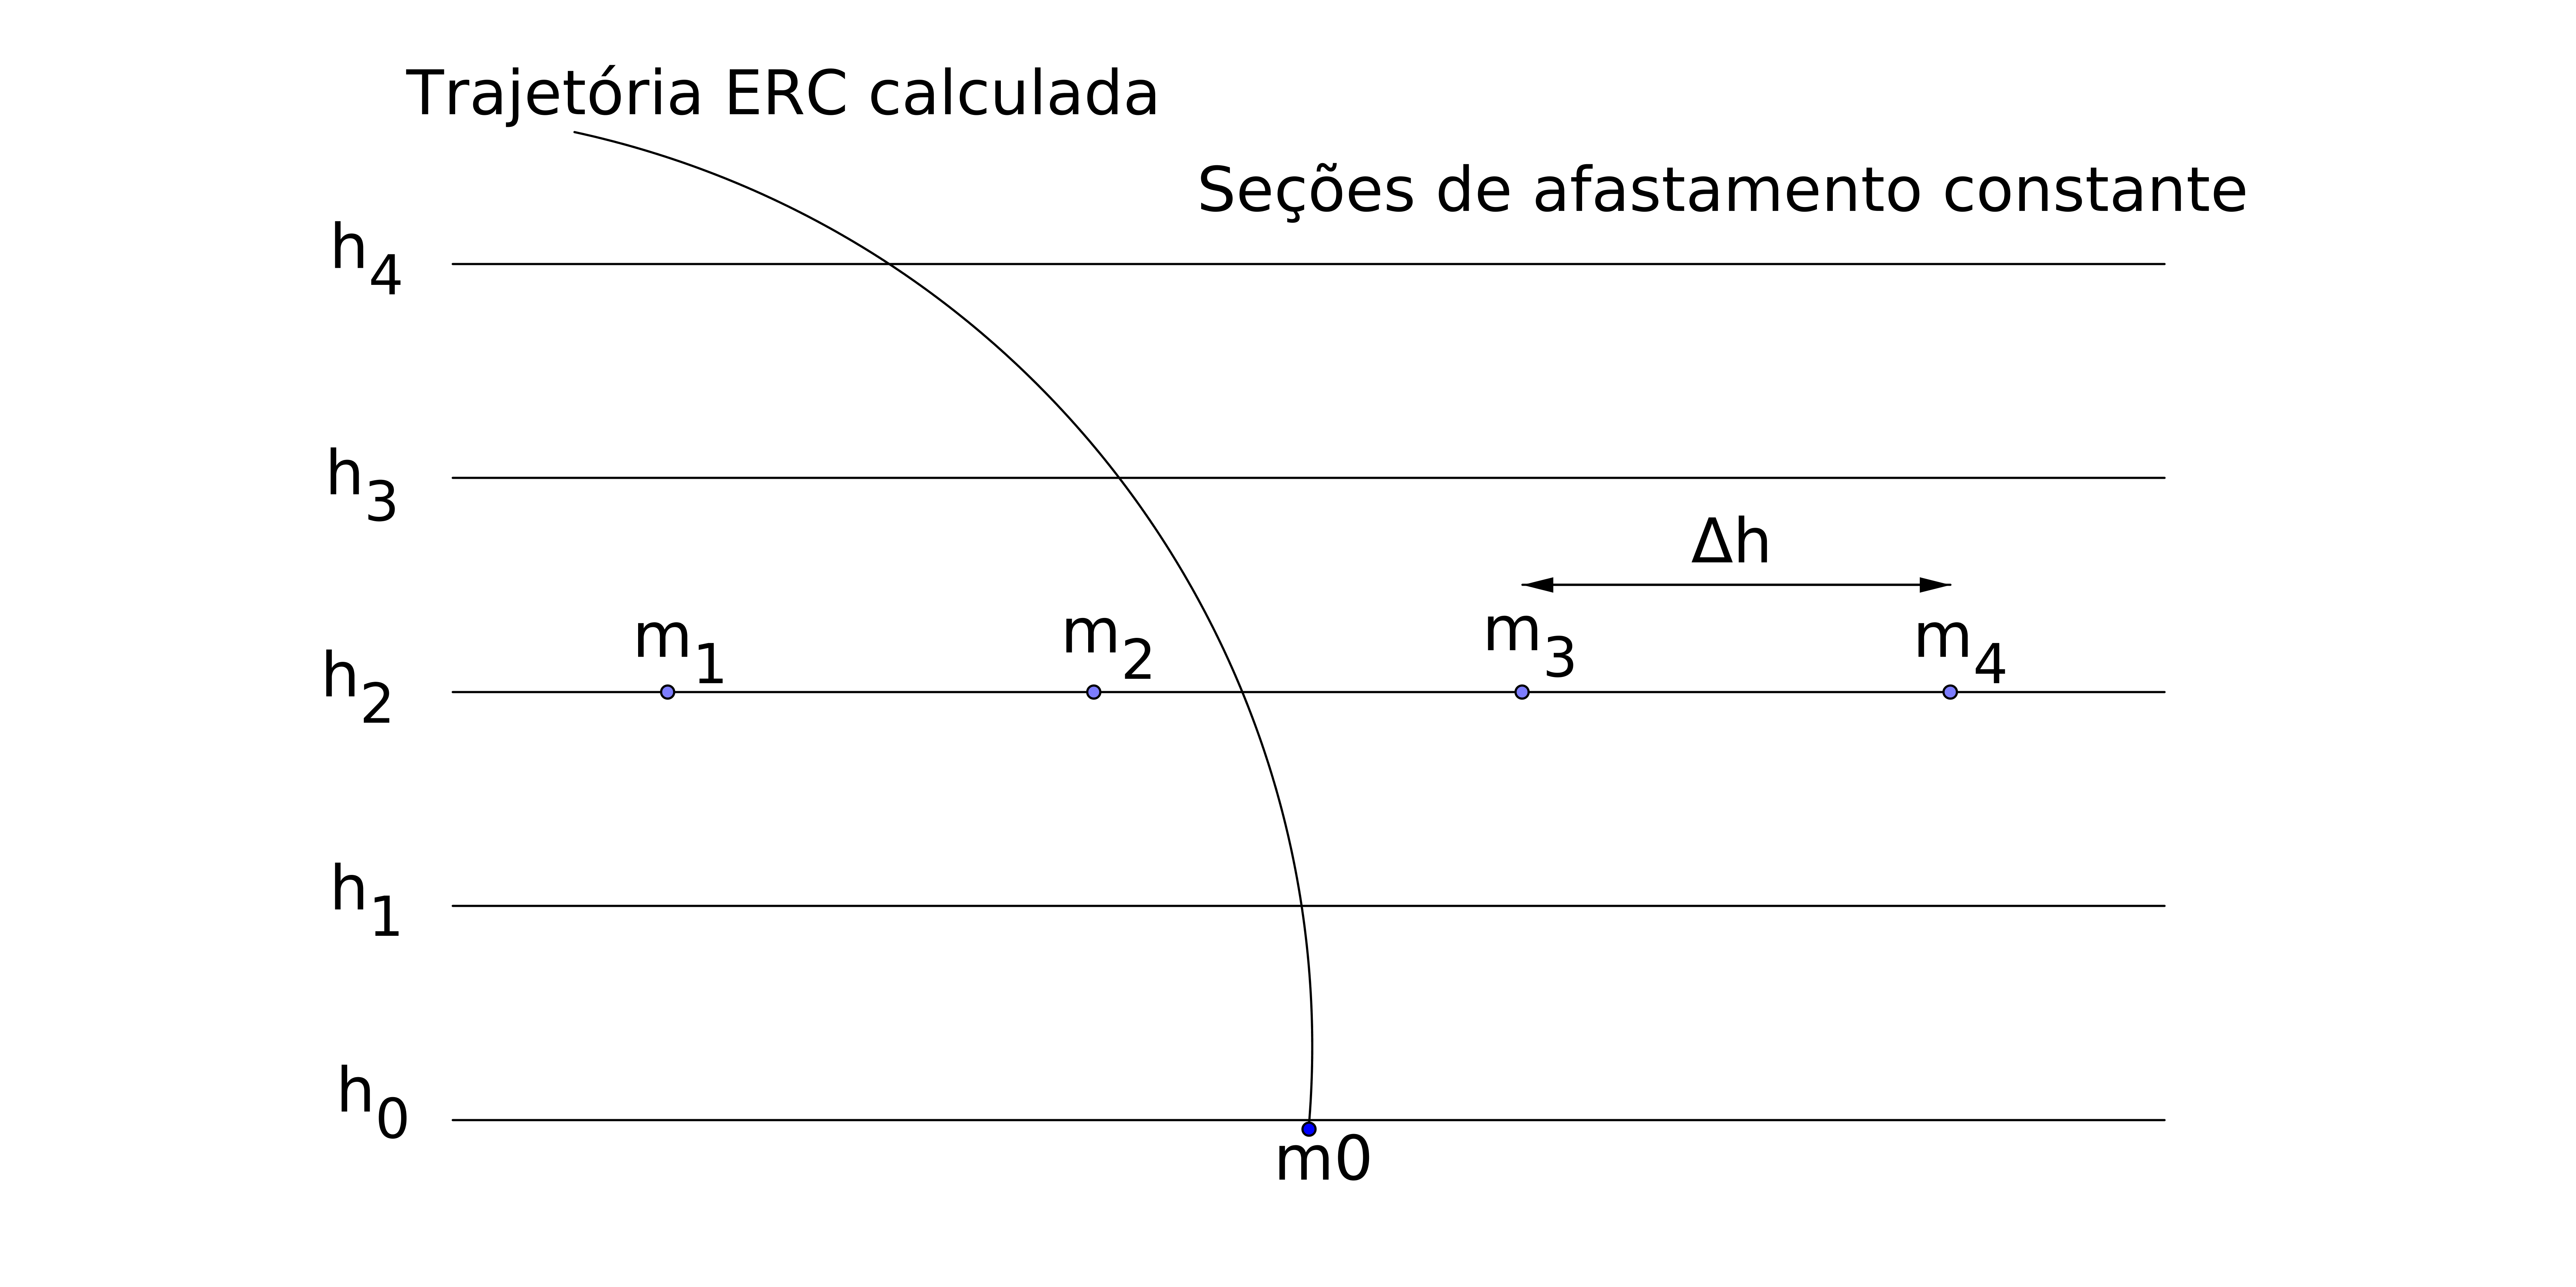
\includegraphics[scale=0.15]{images/interpolacao0.png}
\vspace{-0.3cm}
\end{center}
\begin{center}
 Fonte: Do Autor.
\end{center}
\label{fig:4.1}
\end{figure}


\begin{figure}
\caption{Representação esquemática das seções de afastamento constante após a interpolação. A discretização foi aumentada
intercalando traços zerados $m'_i$ entre os traços originais e depois realizando a interpolação FPE. O traço sísmico 
identificado pela coordenada $m'_2, h2$ está mais próximo da coordenada real da trajetória ERC calculada que os traços 
originais $m_2, h2$ e $m_3, h2$. o processo de interpolação é repetido até que a discretização seja suficiente para amostrar a 
trajetória ERC.}
\begin{center}
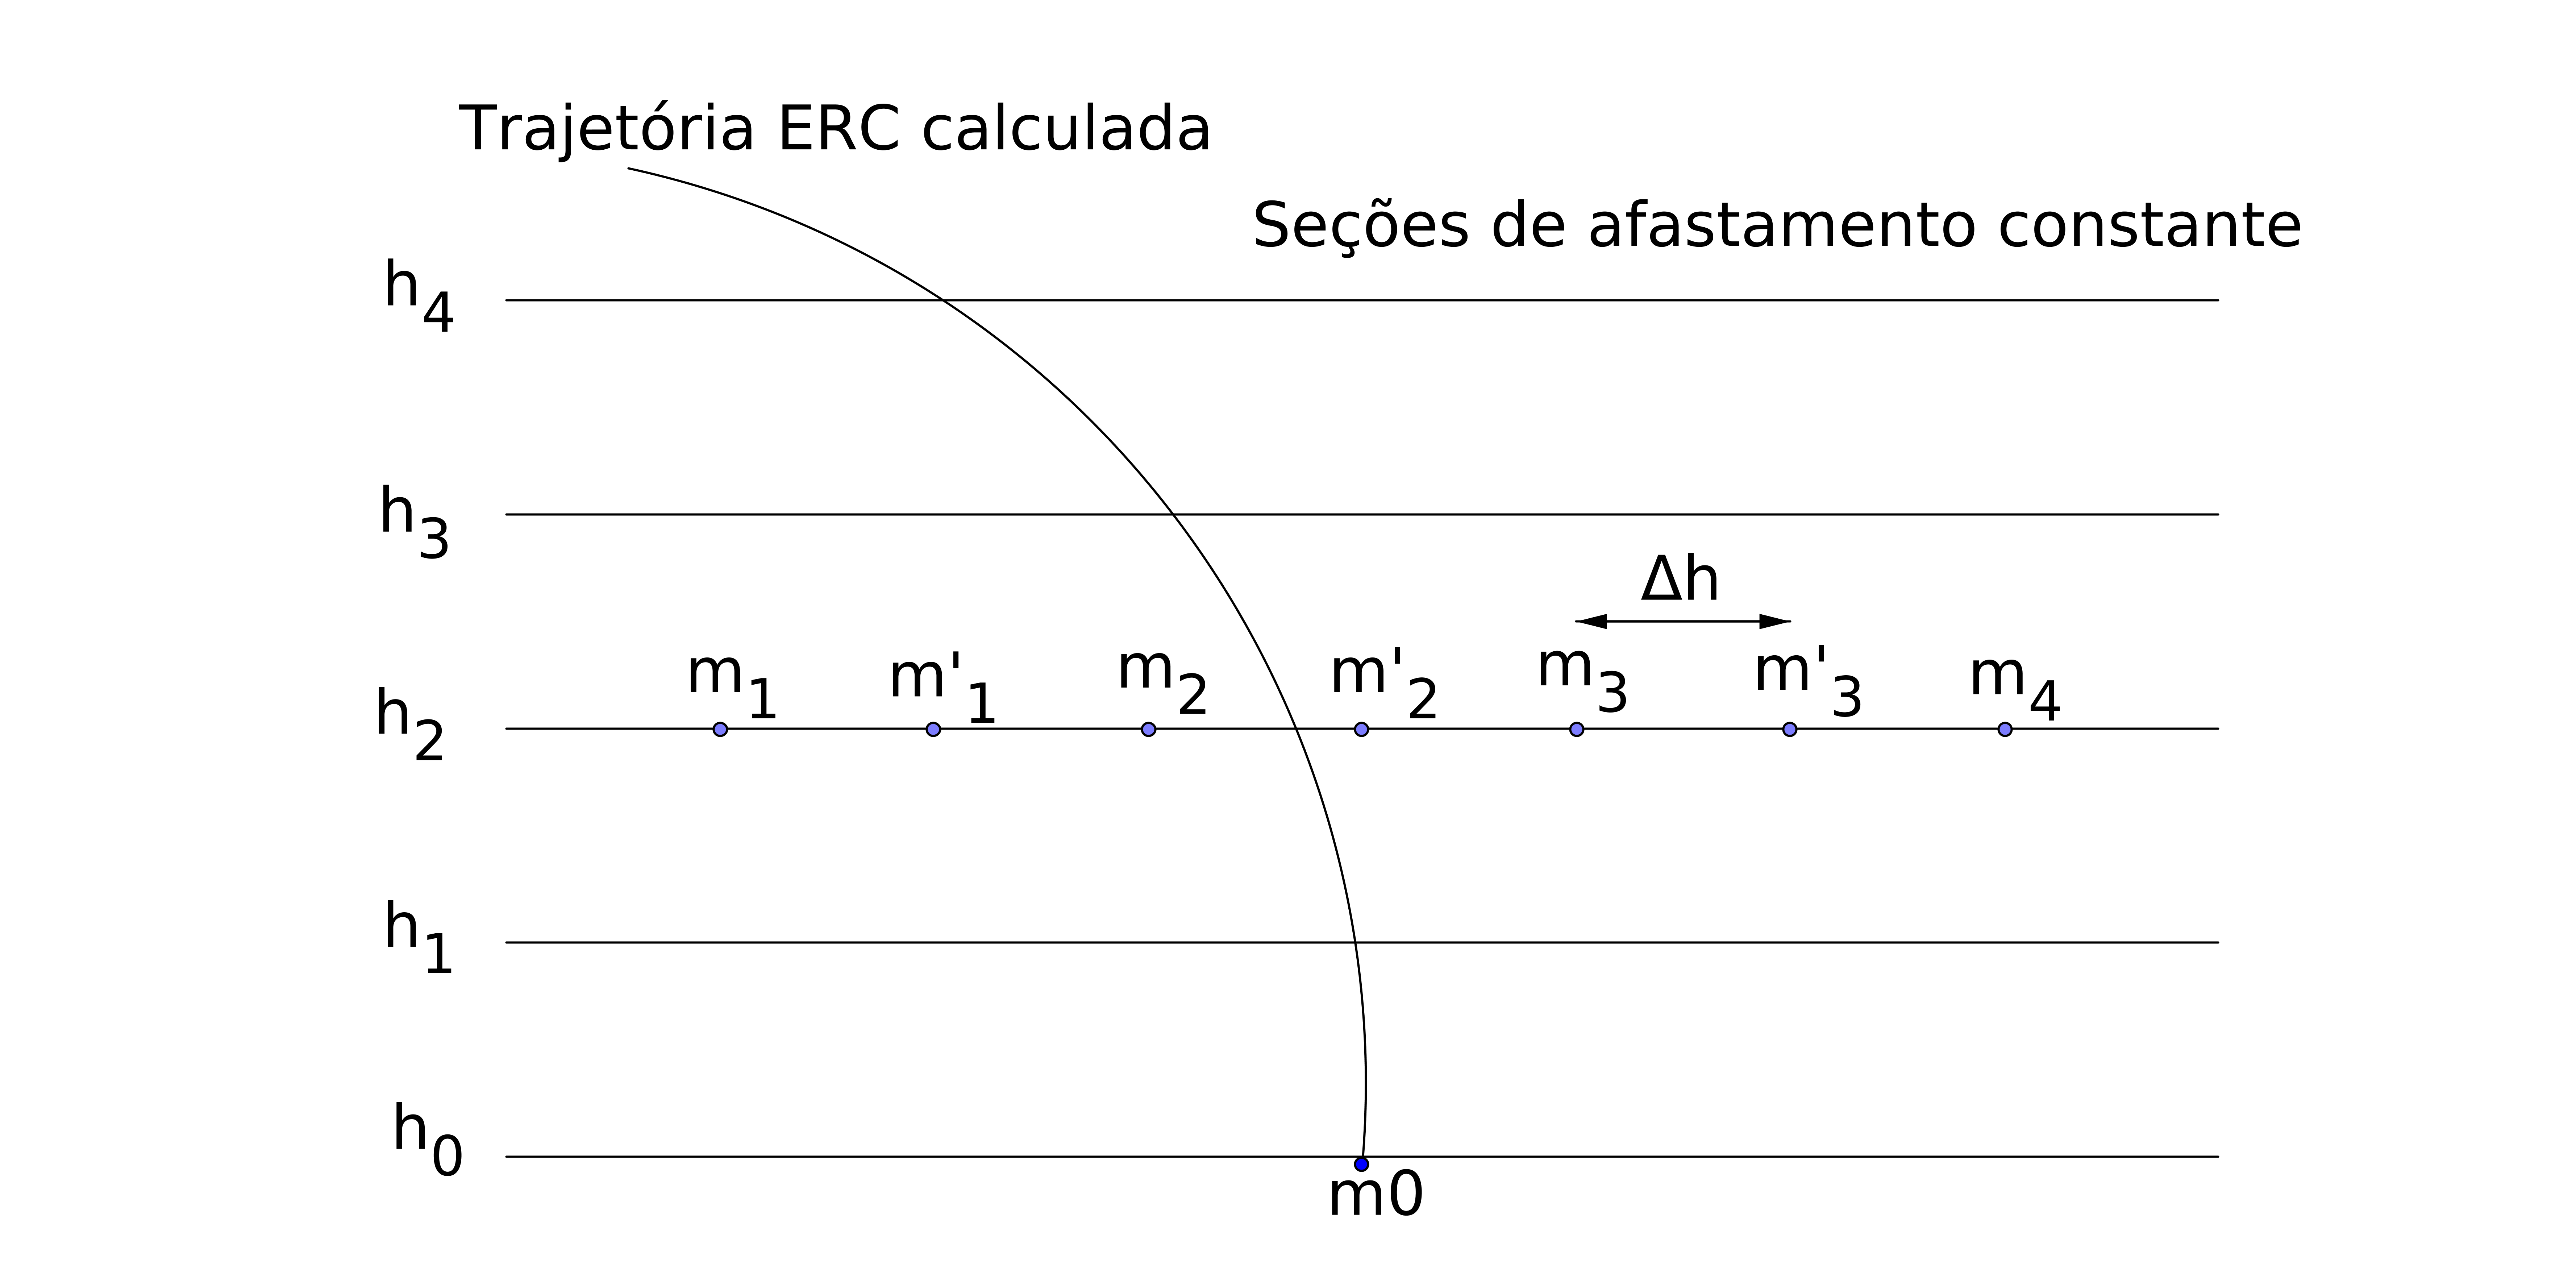
\includegraphics[scale=0.15]{images/interpolacao.png}
\vspace{-0.3cm}
\end{center}
\begin{center}
 Fonte: Do Autor.
\end{center}
\label{fig:4.2}
\end{figure}

